\section{Analysis} % 60-70% (1800-2100 words)

\subsection{Federal inaction as an engine for sub-national innovation}

As was outlined by Harrison, the US federal government has many veto
players due to the fact that legislation must be approved by the
House, the Senate and the President. The high likelihood of veto,
combined with the fact that individual politicians often vote to
protect the business interests of their local constituents rather than
along party lines, means that the US Federal Government's record on
climate issues is weak, and where legislation was successfully passed,
it was often been quickly repealed after a change in
administration~\citep{harrison2010united}.

Although the lack of federal action on climate change paints a picture
of climate apathy in favour of economic growth, it belies a large
segment of the US population who have consistently felt that climate
change is a pressing and urgent concern above that of business, as
illustrated in Figure~\ref{fig:env-vs-econ}. As such, there has been
significant effort to channel the demand for action on climate change
to levels of the governance hierarchy where the systemic barriers to
effective action are not as strong. Efforts include protests against
Siemens\footnote{Who have been associated with the construction of new
  coal power plants~\citep{dw2020,greenpeace2020}.}, the Fridays for
Future organization\footnote{Fridays for Future was started when
  activist Greta Thunberg, started protesting in front of the Swedish
  parliament every school day, and has now morphed into a movement of
  strikes involving over 13 million people~\citep{fff}.}, The Net-Zero
Asset Owners
Alliance\footnote{\url{https://www.unepfi.org/climate-change/united-nations-convened-net-zero-asset-owner-alliance/}},
the We Are Still In
Movement\footnote{\url{https://www.wearestillin.com/}}, and many more.

\begin{figure}[h!]
  \begin{center}
    \begin{tikzpicture}
      \begin{axis}[
          xlabel=Year,
	  ylabel=Percentage,
          ymin=0,
          ymax=100,
	  title={Public Opinion: environment vs economy},
          align=center,
	  grid=both,
          x tick label style={/pgf/number format/.cd,%
          scaled y ticks = false,
          set thousands separator={},
          fixed},
	  minor grid style={gray!25},
	  major grid style={gray!25},
	  width=0.75\linewidth,
          title style={align=left},
          legend style={at={(0.5,-0.15)},anchor=north},
	  %no marks,
          ]
        \addplot[line width=1pt,solid,color=olive] %
	  table[x=year,y=environmental_protection,col sep=comma]{data.csv};
        \addlegendentry{\% Protection of the environment};
        \addplot[line width=1pt,dotted,color=black] %
          table[x=year,y=economic_growth,col sep=comma]{data.csv};
        \addlegendentry{\% Economic growth};
      \end{axis}
    \end{tikzpicture}
    \caption{American respondents were asked which of these statements
      they most you agreed with; ``\textit{Protection of the
        environment should be given priority, even at the risk of
        curbing economic growth}'' or ``\textit{Economic growth should
        be given priority, even if the environment suffers to some
        extent}``~\citep{gallup}}
    \label{fig:env-vs-econ}
  \end{center}
\end{figure}


The model of cooperative federalism employed in the United States
diffuses authority between the federal government and individual state
governments, which leaves room for individual states to legislate on
climate issues. This flexibility has been put to great use in states
such as California\footnote{California's climate programmes, pledges
  and goals span finance, power generation, transportation,
  efficiency, natural resource management, adaptation and
  resilience~\citep{wearestillin-california}}, Connecticut\footnote{In
  Connecticut, `Public Act 08-98, An Act Concerning Connecticut Global
  Warming Solutions' requires the state to achieve an 80\% GHG
  emissions reduction from 2001 levels by
  2050~\citep{wearestillin-connecticut}.}  and Hawai'i\footnote{Hawai'i
  has committed to sourcing 100\% of its net electricity sales from
  renewables by 2045~\citep{wearestillin-hawaii}.} in order to generate
and implement novel climate legislation, a phenomena described as
\textit{compensatory federalism}~\citep{balthasar2019energy}.

Yet elected government is not the only arena in which global warming
is a hotly debated, in-demand and hugely consequential topic. As
Executive Secretary of the UNFCCC Patricia Espinosa writes in a
foreword to Microsoft's white paper on carbon neutrality, a concerted
and polycentric approach from all levels of the governance hierarchy
is required to field an effective response to global warming:

\begin{displayquote}
  This transformation cannot be achieved by governments alone, no
  matter how closely national policies and national action plans align
  with international cooperation. It will only work if all sections of
  society—from local and regional governments to business, investors,
  and citizens—also contribute at increasing levels of scale and
  acceleration.

  -- Patricia Espinosa, Executive Secretary, UNFCCC,
  2016~\citep{microsoft2015}
\end{displayquote}

\subsection{The features of polycentric governance}

Corporate action within the US will now be examined in the context of
the four polycentric governance conditions outlined by Dorsch and
Flaschland; self-organization, site-specific conditions,
experimentation, and learning and trust~\citep{dorsch2017polycentric}.

% Link to the 4 polycentric governance characteristics

\subsubsection{Self-organization}

% Each company is soverign to itself, and acts in the intersts of its
% stakeholders Longer term interests of a company and industry are
% aligned with its image Also aligned with sustainability

Each private company is sovereign to itself, in the sense that board
members, managers, executives and other members of the administrative
structure of the company wield the power to make business decisions on
its behalf. As such, these actors within companies have the authority
to make decisions in the best interests of the company, this includes
obvious actions such as abiding by the law and ensuring profitability,
but also in order to maintain a good social standing for the company
within society.

% Large investors (e.g. Larry Fink of Black Rock) set incentives

Recent moves my large investors indicate that the risk of climate
change is starting to become a credible threat to the long-term
sustainability of many businesses. Larry Fink, the CEO of Black Rock,
the world's largest asset manager recently released a letter warning
companies that climate risk is investment risk, and predicting a
significant reallocation of capital towards sustainable
investments~\citep{reshaping2020fink}. Fink's letter is significant,
since the opinion of massive institutional investors such as Black
Rock sets the tone of conversation at the executive level of
business\footnote{Soon after the letter was released, many companies
  released sustainability reports. Some had large commitments such as
  Delta, which pledged to spend \$1bn over ten years on sustainability
  and to become carbon neutral, but others appear to be at risk of
  greenwashing. As outlined by~\citep{parguel2011sustainability},
  sustainability ratings could be used to deter companies from
  greenwashing.}, and hints that companies with large exposures to
risks related to climate change (such as having lots of stranded
assets) could be seen as less attractive investments in the future.

% Private regulation & certification initatives provide a path forward
% Explicitly call out public policy failures here (bottom of page 398
% and 399, bottom of page 403 on Auld and Gulbrandsen)

As stated by Auld and Gulbrandsen, the environmental and social
reputations of any given company reflect on the entire industry of
which it is part, and as such, there is often peer pressure among
companies to maintain a good social standing. This incentivises the
creation of private regulation, where ``non-state actors set rules to
govern the behaviour of others'', and thereby forming a
self-governing, self-policing and self-organizing mechanism to ensure
that companies are acting in each-other's
interests~\citep{auld2013private}.

They also explicitly call out the public policy failures of the
international climate regime as a demand factor in the generation of
climate related private regulation, showing how the corporate sector
can self-organize as a direct response to a lack of higher-level
governance~\citep[p.403]{auld2013private}. Cashore describes this form
of private regulation as Non-State Market Driven Governance Systems
(NSMD), and shows that it is most prevalent in the fields of
responsible environmental and social management practices
~\citep{cashore2002legitimacy}.

% Specifically: Renewable Energy Buyers Alliance (Google helped found
% & joined)
% blog.google/outreach-initiatives/sustainability/cop25-every-business-protect-our-planet/

In the field of private climate regulation, long-standing projects
such as the Carbon Disclosure
Project\footnote{\url{https://www.cdp.net/en}} (which was founded in
2000, and seeks to audit companies on a range of climate related
measures) are well established and provide essential services that
governments and legislators are not providing, though it has been
shown that companies do not always respond to their
efforts~\citep{matisoff2013convergence}.

Despite this, newer projects such as \textit{Renewable Energy Buyers
  Alliance (REBA)} continue to form, providing ever more specialised
private regulation as interest grows and the sector expands. Founded
in 2017, the REBA facilitates private companies' procurement of
renewable energy across the United States, in spite of lackluster
federal support for an energy transition~\citep{reba2020}.

\subsubsection{Site-specific conditions}

% Each industry is different
% Airlines - Delta
% Technology - environment.google, microsoft

One major difficulty in dealing with wicked problems such as climate
change is their pervasiveness, and the large number of changes across
all of society that must be made in order to tackle them. As Dorsch
and Flachsland show, and as Scott discusses at length in
\textit{Seeing like a State}, actors with a deep level of
understanding of a given situation are best equipped to exploit local
synergies, achieving a solution that is more optimal than could be
reached at a more abstract higher level of
governance~\citep{dorsch2017polycentric,scott1998seeing}.

Both authors show that it is the diversity of context specific
problems that makes the heterogeneity of lower-level governance
structures highly effective. In the case of the corporate sector, each
industry is by definition an `expert' in the field that it operates,
and as such is able to recognise the `site-specific' changes
required in order to create a suitable `polycentric task' to be
implemented.

One industry that has been amenable to a sustainable transition and
exemplifies the notion of highly tailored responses has been the cloud
computing industry, where industry leaders have committed billions of
dollars towards sustainability initiatives and developing renewable
electricity generation.

For example, Google, a large player in the cloud computing industry,
is able to exploit synergies between its business model and a
sustainable transition. According to its environmental report, Google
enters into Purchasing Power Agreements (PPA) with energy companies
which commits it to buying a given amount of renewable energy over a
certain number of years (thus lowering the risk of new green energy
investments and increasing their changes of success), which according
to its report has driven nearly \$5 billion of new capital investment
into renewable energy generation and has played a large part in
enabling Google to be carbon neutral since
2007~\citep{google,google2013}.

Dorsch and Flaschland show that one disadvantage of using lower-level
governance structures to tackle climate change issues, is that
sometimes they don't have the requisite authority to pass
legislation. In some sense, this is very true for corporations, since
cannot pass climate legislation. However, corporations do have almost
absolute power to make changes to their own business practices, and so
are flexible and powerful with regard to their own level of the
governance hierarchy.

Yet counter examples to Dorsch and Flaschland's assertion exist,
showing that legislative issues can be overcome by corporate actors
through lobbying. For example, when Google was unable to implement its
PPA strategy inside the existing legal framework of Taiwan, it
successfully lobbied for a legislative amendment to the Electricity
Act which lifted restrictions on direct purchases of electricity if
the electricity comes from renewable sources~\citep{taiwan}. This is
evidence of Google acting as a policy entrepreneur to facilitate
policy diffusion, in this case, to help bring the practice of
corporate direct energy purchases from the United States and Europe
into the Taiwanese energy market.

\subsubsection{Experimentation and learning}

`Experimentation and learning', the third criteria outlined by Dorsch
and Flaschland easily maps onto the competitive aspects of the
corporate world. Corporate competition drives innovation, and an
innovation by one company is often adopted as quickly as possible by
its competitors.

% Microsoft is the first large company to pledge negative emissions
% Google uses its AI expertise to optimise its datacenters
% https://www.blog.google/inside-google/infrastructure/safety-first-ai-autonomous-data-center-cooling-and-industrial-control/

Another cloud computing company, Microsoft, can also be seen to engage
in polycentric experimentation. In January 2020, Microsoft announced
that it would be ``carbon negative'' by 2030 (shown in
Figure~\ref{fig:microsoft}), announced a \$1 billion dollar climate
innovation fund, and committed to removing all its historical carbon
emissions by 2050. This investment makes Microsoft the first company
in the world to commit to being carbon negative, and is undoubtedly a
commercial and financial experiment, though it is too early to tell if
other companies will follow suit.

To achieve its goal, Microsoft will buy energy from 100\% renewable
sources by 2025, applying an internal carbon tax of \$15 per metric
ton. Microsoft intends to remove carbon from the atmosphere using a
variety of methods, described as ``\textit{potentially including
  afforestation and reforestation, soil carbon sequestration,
  bio-energy with carbon capture and storage (BECCs), and direct air
  capture (DAC)}''~\citep{microsoft}.

\begin{figure*}[h]
  \begin{center}
    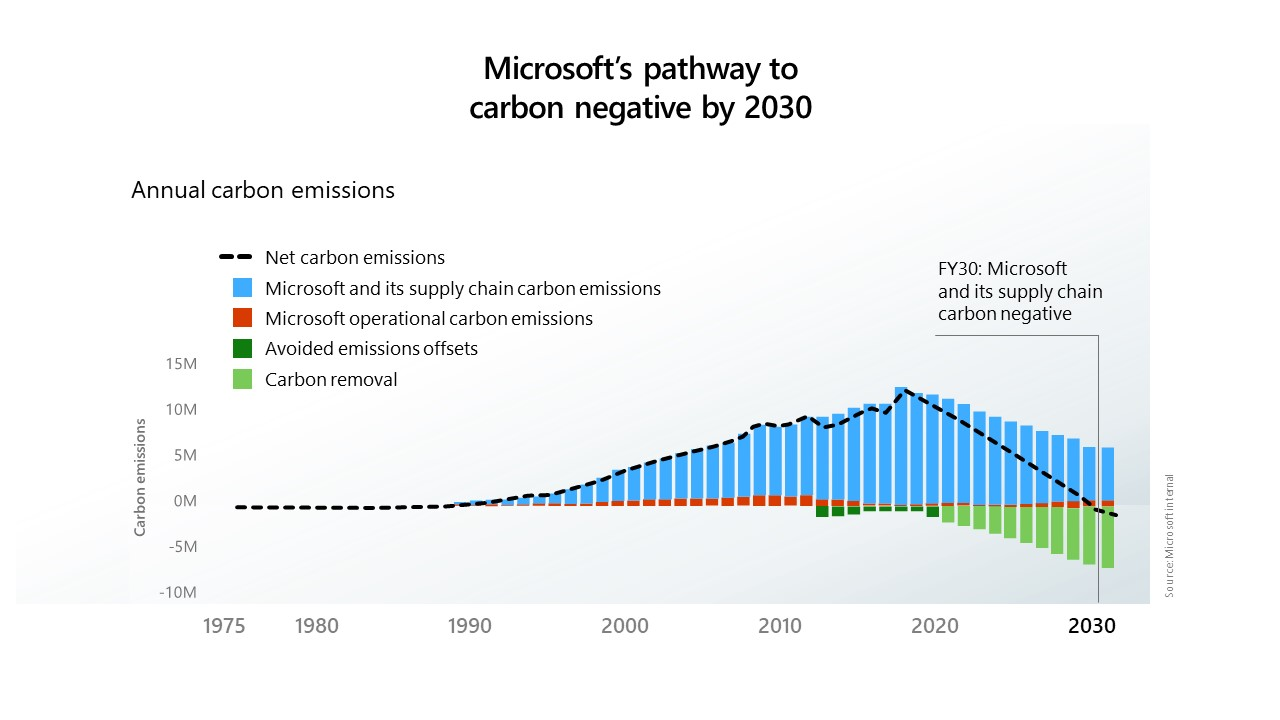
\includegraphics[width=\linewidth]{microsoft-sustainability.jpg}
    \caption{A graph showing the carbon emissions of Microsoft
      (including the negative emissions that were avoided using
      offsets), and showing the intended path towards net zero, and
      then negative emisisons from 2030~\citep{microsoft}.}
    \label{fig:microsoft}
  \end{center}
\end{figure*}


% Experiments must fit the site specific conditions

% Learning between certification & self regulation initatives (see
% paper on private regulation)

In their paper on private regulation in global environmental
governance, Auld and Gulbrandsen show how private regulation can
facilitate the adoption of standards through peer pressure, providing
a path for polycentric learning~\citep{auld2013private}. Likewise, it
has been demonstrated in Business Management literature that
corporations engage in `diffusion', defined as ``the process by which
innovations spread to the members of a social system over
time''~\citep{rogers1979diffusion}, and that corporations will
actively search their environment to find solutions to meet their
organizational problems~\citep[p.371]{rogers2010diffusion}.

\subsubsection{Trust}

% Trust is not the same as blind faith, where parties simply sit down
% and ‘do the right things’ according to someone’s moral
% compass. Rather, trust is earned by mutual commitments that are not
% overly costly to monitor -
% https://www.repository.law.indiana.edu/cgi/viewcontent.cgi?article=2415&context=facpub
% Private regulation and certification increases trust

% Ostrom says: "an asset that individuals build over time by engaging
% in mutually beneficial transactions that cannot be consummated in an
% immediate quid pro quo exchange"
% (https://www.repository.law.indiana.edu/cgi/viewcontent.cgi?article=2415&context=facpub)

According to Cole, Ostrom's view on trust is that it must be
\textit{mutually earned} by actions that can be verified by the
different parties interacting in a
system~\citep{cole2015advantages}. A mechanism for establishing trust
in the context of private business is outlined by Auld and
Gulbrandsen, specifically private certification, which facilitates
trust through differentiating responsible companies from irresponsible
companies~\citep[p.396]{auld2013private}, which in turn, is built on
the general framework that Ostrom outlines for building trust. Taking
a game theoretic view, Ostrom asserts that through mutually beneficial
interactions, a stock of trust is built between parties over time,
seeing the interactions as one long `game' rather than many individual
exchanges~\citep{bromley1992making}.

This mechanism of trust building is evident in the wide range of
private organizations within the corporate sector that facilitate
certification, and are widely recognised as being authoritative within
their sphere of influence. Examples include The Forest Stewardship
Council\footnote{The FSC promotes environmentally appropriate,
  socially beneficial, and economically viable management of the
  world’s forests, and operates in over 90 countries~\citep{fsc}. It
  is called out by Cashore as a particularly effective non-state
  market driven governance actor~\citep{cashore2002legitimacy}.}, The
Marine Stewardship Council\footnote{The MSC runs certification
  programmes for sustainable fishing, and certifies around 15\% of
  fish catches~\citep{msc, auld2013private}.}, and the Fairtrade
Labelling Organization\footnote{The Fairtrade Labelling Organization
  certifies products as having supply chains that give decent and more
  fair working conditions for farmers and workers, particularly in
  developing countries, and according to its website, has a reach of
  over 1.6 million workers~\citep{fairtrade,
    auld2013private}.}. Pargue et al. explain how these types of
monitoring organizations can be used to help build both consumer trust
and inter-corporation trust by certifying that the sustainability
practices of companies are legitimate and effective, and thus
preventing free-riders and
greenwashing~\citep{parguel2011sustainability}.

\subsection{Corporate Laggards}

This paper has focused on climate-leaders in the corporate world, yet
laggards exist on the opposite end of the spectrum. A particularly
well studied case is that of the oil industry, where there was
widespread acknowledgment of the problem of anthropogenic climate
change among oil industry executives at least a decade before it was
brought to the attention of the US government~\citep{franta2018early}.

In modern times, climate malfeasance in the corporate arena continues
to thrive; companies involved in the production of fossil fuels have
been shown to have purposefully misled the public through advertising
campaigns~\citep{supran2017assessing}, business lobby groups act as
policy entrepreneurs and push policies that preserve the
status-quo~\citep{goldenberg2013secret} and companies engage in
greenwashing, which lets them claim to be environmentally conscious,
while making few changes that actually reduce their
footprint~\citep{bruno1997world}.

Thus, the question of how the policies and strategies of corporate
laggards will evolve over time remains. As described by Shipan and
Volden, will policies ``snowball'', and diffuse throughout the wider
business world, or will they act as a ``pressure valve'' and make
government level action to force laggards to act less
important~\citep{shipan2012policy}?  Further work is required to answer
these questions.

% Draw heavily on the ideas in the "Private Regulation in
% Environmental Governance" paper

